% 自然解剖插画仅提供脑形态；全部区域定位与通路由 TikZ 精确叠加。
% 点位为教学投影而非实测区域边界；V1 内侧位置由右侧视图说明。
% 位置：Wandell et al. (2007), doi:10.1016/j.neuron.2007.10.012。
% 通路：Purves et al. (2001), Neuroscience；Goodale & Milner (1992)。
\begin{tikzpicture}[x=1mm,y=1mm,font=\figurefont\footnotesize,
  area/.style={circle,minimum size=2.5mm,inner sep=0pt,draw=FigureInk,fill=white},
  annotation/.style={fill=none,inner sep=0.7mm},
  ventral/.style={book arrow,draw=FigureRed,line width=1.7pt,
    preaction={draw=white,line width=3.5pt}},
  dorsal/.style={book arrow,draw=FigureBlue,line width=1.7pt,dashed,
    preaction={draw=white,line width=3.5pt}},
  leader/.style={draw=FigureMuted,line width=0.5pt}]
  \node[anchor=south west,inner sep=0pt] at (0,0)
    {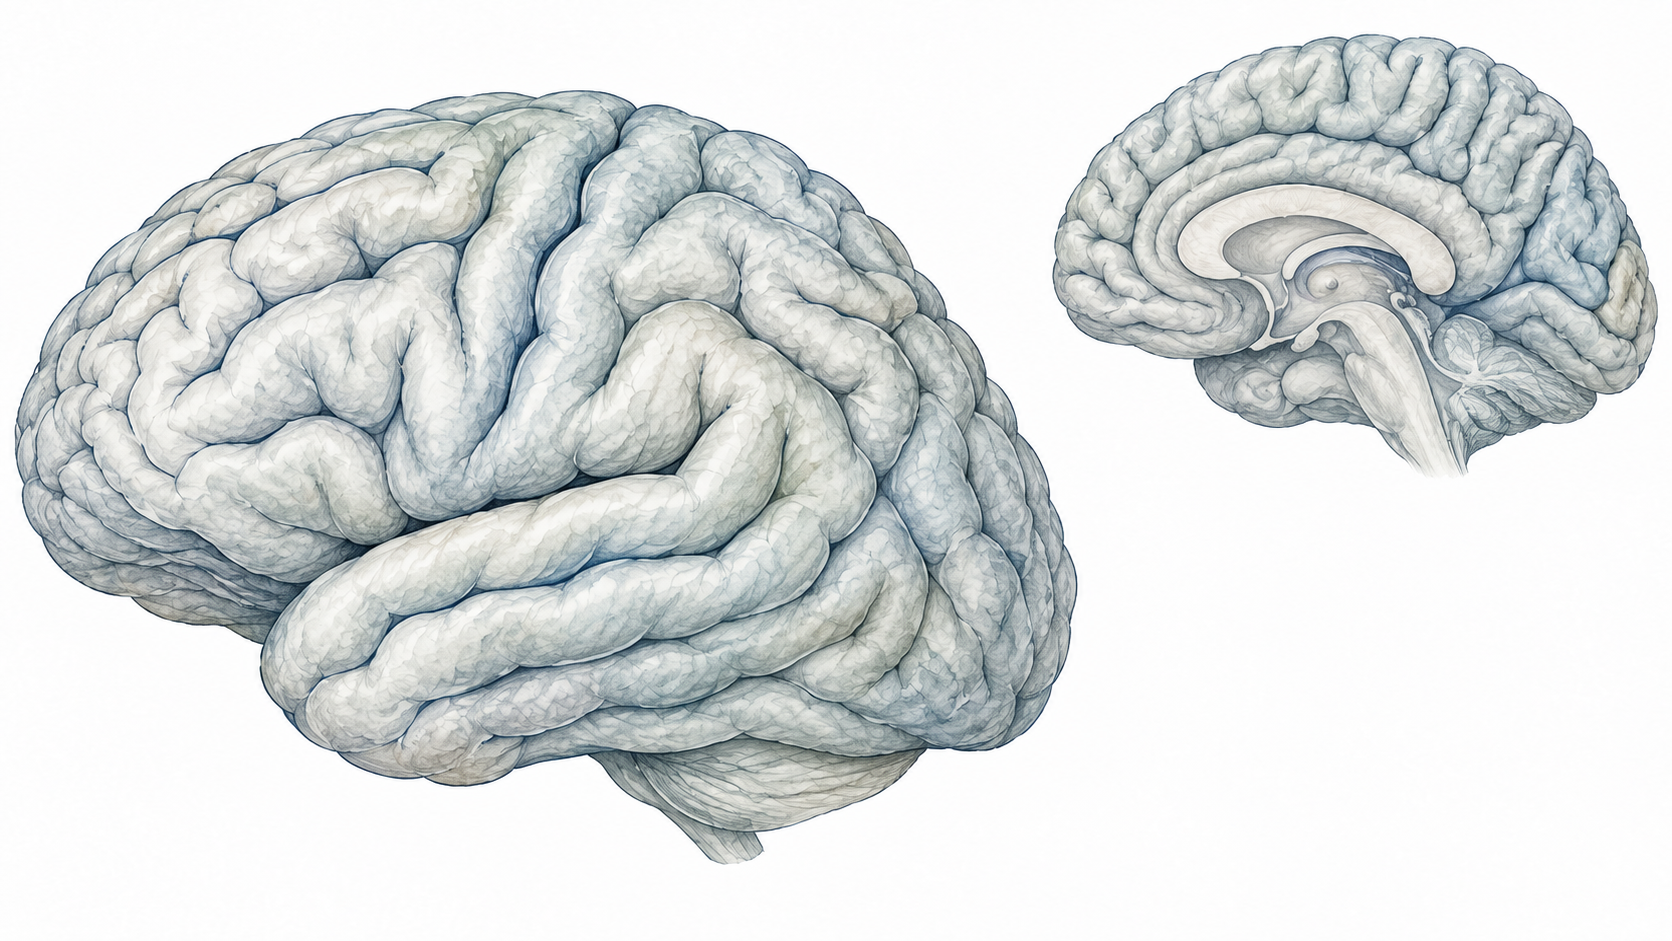
\includegraphics[width=168mm]{figures/03-models/02-neural-network-models/generated/neural-overview-brain-anatomy.png}};
  \node[anchor=west,text=FigureMuted] at (1,100) {外侧视图：左为前，右为后};
  \node[text=FigureMuted] at (138,100) {内侧视图};
  \node[annotation] (central) at (49,94) {中央沟};
  \draw[leader] (central.south)--(54,85)--(57,72);
  \node[annotation,text=FigureMuted] at (23,66) {额叶};
  \node[annotation,text=FigureMuted] at (38,34) {颞叶};
  \node[annotation,text=FigureMuted] at (103,33) {枕叶};
  \node[area,draw=FigureBlue] (parietal) at (74,70) {};
  \node[annotation] (parietallabel) at (81,90) {顶叶皮层};
  \draw[leader] (parietallabel.south)--(81,81)--(parietal);
  \node[area] (v1) at (103,42) {};
  \node[annotation,anchor=west] (v1label) at (111,43) {V1（内侧投影）};
  \draw[leader] (v1)--(v1label.west);
  \node[area] (v2) at (97,46) {};
  \node[annotation] (v2label) at (110,53) {V2};
  \draw[leader] (v2)--(103,49)--(v2label.west);
  \node[area] (v3) at (97,59) {};
  \node[annotation] (v3label) at (102,80) {V3（背侧）};
  \draw[leader] (v3label.south)--(99,73)--(v3);
  \node[area] (mt) at (81,42) {};
  \node[annotation] (mtlabel) at (73,32) {MT（V5）};
  \draw[leader] (mtlabel.north)--(77,38)--(mt);
  \node[area] (v4) at (90,25) {};
  \node[annotation] (v4label) at (96,7) {V4／hV4};
  \draw[leader] (v4label.north)--(94,17)--(v4);
  \node[area] (it) at (57,25) {};
  \node[annotation] (itlabel) at (47,7) {下颞皮层IT};
  \draw[leader] (itlabel.north)--(51,16)--(it);
  \draw[book arrow] (v1)--(v2);
  \draw[dorsal] (v2) to[out=105,in=-70] (v3);
  \draw[dorsal] (v3) to[out=165,in=-5] (parietal);
  \draw[dorsal] (v2) to[out=185,in=20] (mt);
  \draw[dorsal] (mt) to[out=100,in=-70] (parietal);
  \draw[ventral] (v2) to[out=-100,in=70] (v4);
  \draw[ventral] (v4) to[out=185,in=-5] (it);
  % 内侧图：距状沟的后部两岸属于 V1 的主要位置。
  \draw[FigureYellow,line width=1.1pt] (151,64) to[out=-10,in=150] (163,61);
  \node[area,draw=FigureYellow] (v1medial) at (159,66) {};
  \node[annotation] (v1mediallabel) at (145,76) {V1};
  \draw[leader] (v1mediallabel.south)--(150,69)--(v1medial);
  \node[annotation] (calcarine) at (145,44) {距状沟};
  \draw[leader] (calcarine.north)--(152,55)--(157,62.5);
  \path[draw=FigureGrid,fill=white,rounded corners=1mm,line width=.6pt]
    (117,3) rectangle (168,39);
  \node[font=\figurefont\footnotesize] at (142.5,36) {抽象路径};
  \foreach \x/\label in {124/{V1/V2},142/V4,160/IT}{
    \node[draw=FigureRed,fill=white,rounded corners=.6mm,
      minimum width=12mm,minimum height=7mm,inner sep=.5mm] (v-\x)
      at (\x,28) {\label};
  }
  \draw[ventral] (v-124)--(v-142);
  \draw[ventral] (v-142)--(v-160);
  \foreach \x/\label in {124/{V1/V2},142/MT,160/顶叶}{
    \node[draw=FigureBlue,fill=white,rounded corners=.6mm,
      minimum width=12mm,minimum height=7mm,inner sep=.5mm] (d-\x)
      at (\x,13) {\label};
  }
  \draw[dorsal] (d-124)--(d-142);
  \draw[dorsal] (d-142)--(d-160);
  \node[anchor=west,text=FigureInk] at (118,21) {内容what};
  \node[anchor=west,text=FigureBlue] at (118,6) {空间where};
\end{tikzpicture}
